\documentclass[12pt]{article}
\usepackage{graphicx}
\usepackage{amsmath}
\usepackage{minted}
\usepackage{multicol}
\usepackage{subcaption}
\usepackage[english]{babel}
\usepackage{placeins}

\title{Modular Exponentiation and Binary Arithmetic in Python.}
\author{Md Tajim An Noor}
\date{}
\begin{document}
\vspace*{\fill}
\begin{center}

    \emph{Heaven's Light is Our Guide} \\
    \textbf{Rajshahi Universiy of Engineering and Technology} \\

    \begin{figure}[H]
        \centering
        
\includegraphics[scale=.34]{images/RUET_logo.png}
        \label{fig:ruet_logo}
    \end{figure}
    \vspace{5mm}

    \textbf{Course Code}\\
    ECE 2214\\
    \vspace{3mm}
    \textbf{Course Title}\\
    Numerical Methods and Discrete Mathematics Sessional

    \vspace{5mm}
    \textbf{Experiment Date:} October 14, 2023,\\
    \textbf{Submission Date:} {November 4, 2023}\\

    \vspace{5mm}
    \textbf{Lab Report 6:} Finding Chinese remainder theorem \& Carmichael number using python

    \vspace{15mm}

    \begin{tabular}{c|c}
        \textbf{Submitted to} & \textbf{Submitted by} \\
        Md. Nahiduzzaman      & Md. Tajim An Noor     \\
        Lecturer              & Roll: 2010025         \\
        Dept of ECE, Ruet     &                       \\
    \end{tabular}

\end{center}
\vspace*{\fill}

\pagebreak

\tableofcontents

\maketitle
\section{Introduction}


\subsection{Chinese Remainder Theorem}
The Chinese remainder theorem, named after the Chinese heritage of problems involving systems of linear congruences, states that when the moduli of a system of linear congruences are pairwise relatively prime, there is a unique solution of the system modulo the product of the moduli.


\subsection{Carmichael Number}
A composite integer $n$ that satisfies the congruence $b\textsuperscript{n-1}\equiv1\text{ (mod n)}$ for all positive integers $b$ with $gcd(b, n) = 1$ is called a Carmichael number.\cite{rosenDiscrete}


\section{Tools Used}
\begin{itemize}
    \item Python
    \item VS Code - for running python code
    \item MacTeX -\LaTeX  compiler
    \item VS Code with \LaTeX workshop extension as a text editor
\end{itemize}

\section{Process}

\subsection{Code:}
\subsubsection{Chinese Reminder Theorem}
\inputminted[breaklines,linenos]{python3}{codes/chineseRem.py}
\vspace*{40mm}
\subsubsection{Carmichael Number}
\inputminted[breaklines,linenos]{python3}{codes/carma.py}


\vspace{20mm}
\subsection{Output}
\begin{figure}[H]
    \begin{subfigure}{.5\textwidth}
        \centering
        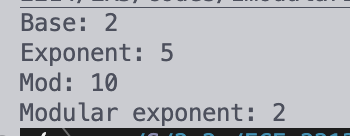
\includegraphics[width=.8\linewidth, height = .73in]{images/output/expo1.png}
        \caption*{}
        \label{fig:expo1}
    \end{subfigure}
    \begin{subfigure}{.5\textwidth}
        \centering
        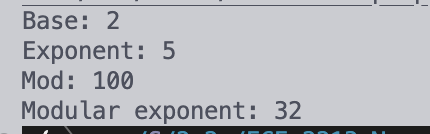
\includegraphics[width=.8\linewidth]{images/output/expo2.png}
        \caption*{}
        \label{fig:expo2}
    \end{subfigure}
    \begin{subfigure}{.5\textwidth}
        \centering
        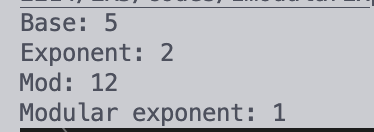
\includegraphics[width=.8\linewidth]{images/output/expo3.png}
        \caption*{}
        \label{fig:expo3}
    \end{subfigure}
    \begin{subfigure}{.5\textwidth}
        \centering
        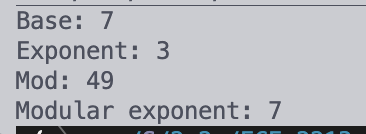
\includegraphics[width=.8\linewidth]{images/output/expo4.png}
        \caption*{}
        \label{fig:expo4}
    \end{subfigure}
    \caption{Outputs for Modular Exponentiation}
    \label{fig:expo}
\end{figure}
\begin{figure}[H]
    \begin{subfigure}{.5\textwidth}
        \centering
        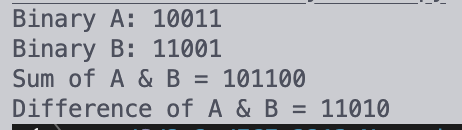
\includegraphics[width=.8\linewidth]{images/output/bin1.png}
        \caption*{}
        \label{fig:bin1}
    \end{subfigure}
    \begin{subfigure}{.5\textwidth}
        \centering
        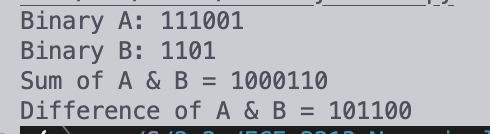
\includegraphics[width=.8\linewidth]{images/output/bin2.png}
        \caption*{}
        \label{fig:bin2}
    \end{subfigure}
    \newline
    \begin{subfigure}{.5\textwidth}
        \centering
        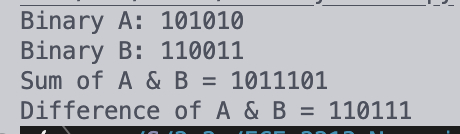
\includegraphics[width=.8\linewidth]{images/output/bin3.png}
        \caption*{}
        \label{fig:bin3}
    \end{subfigure}
    \begin{subfigure}{.5\textwidth}
        \centering
        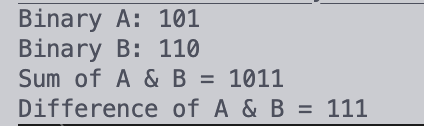
\includegraphics[width=.8\linewidth]{images/output/bin4.png}
        \caption*{}
        \label{fig:bin4}
    \end{subfigure}
    \caption{Outputs for Contraposition}
    \label{fig:bin}
\end{figure}

\begin{figure}[H]
    \begin{subfigure}{.5\textwidth}
        \centering
        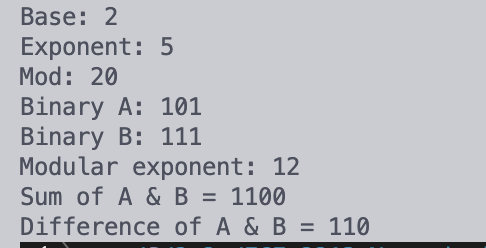
\includegraphics[width=.8\linewidth]{images/output/int1.png}
        \caption*{}
        \label{fig:int1}
    \end{subfigure}
    \begin{subfigure}{.5\textwidth}
        \centering
        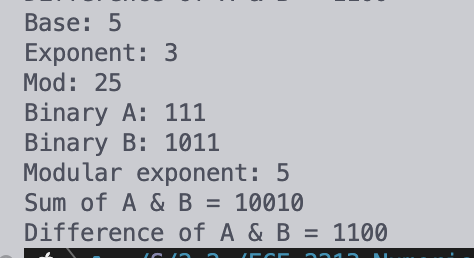
\includegraphics[width=.8\linewidth, height=1.1in]{images/output/int2.png}
        \caption*{}
        \label{fig:int2}
    \end{subfigure}
    \begin{subfigure}{.5\textwidth}
        \centering
        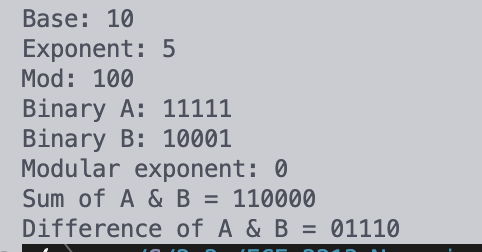
\includegraphics[width=.8\linewidth,]{images/output/int3.png}
        \caption*{}
        \label{fig:int3}
    \end{subfigure}
    \begin{subfigure}{.5\textwidth}
        \centering
        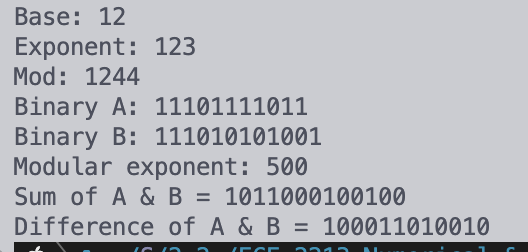
\includegraphics[width=.8\linewidth]{images/output/int4.png}
        \caption*{}
        \label{fig:int4}
    \end{subfigure}
    \caption{Outputs for Logical Equivalence}
    \label{fig:int}
\end{figure}

\section{Discussion}
In the above codes, for the first one there's another way to find the solution. The one used here uses inverse modulo based implementation. Inputs are the three numbers which are pairwise co-prime, and given remainders of these numbers when an unknown number x is divided by them. \cite{chineseCar}\\
For the Carmichael Number problem, we iterate through all numbers from 1 to n and for every relatively prime number, we check if its $(n-1)\textsuperscript{th}$ power under modulo n is 1 or not. \cite{chineseCar}

\bibliographystyle{IEEEtran}
\bibliography{ref}

\end{document}